\section{[Complete] The Screw Axle}

This technique was born out of necessity. Take a screw, put two nuts on it, and screw them in opposite directions so that they clash into one another. With a wrench and a screwdriver, tighten the nuts in opposite directions so that they are tighened by each other's forces. What you have now is a screw axle, where the two nuts acts like a shaft collar.

Screw axles can be used to attached \textit{literally} anything to a metal part strongly while still maintaining a degree of freedom. While these are normally used to make metal whips (steel bars with screw axles), they can be used to secure encoders as well. As encoders require a lot of torque to turn if tightened, securing them with screw axles allow unpowered wheels to turn extremely easily.

\begin{figure}[h]
    \centering
    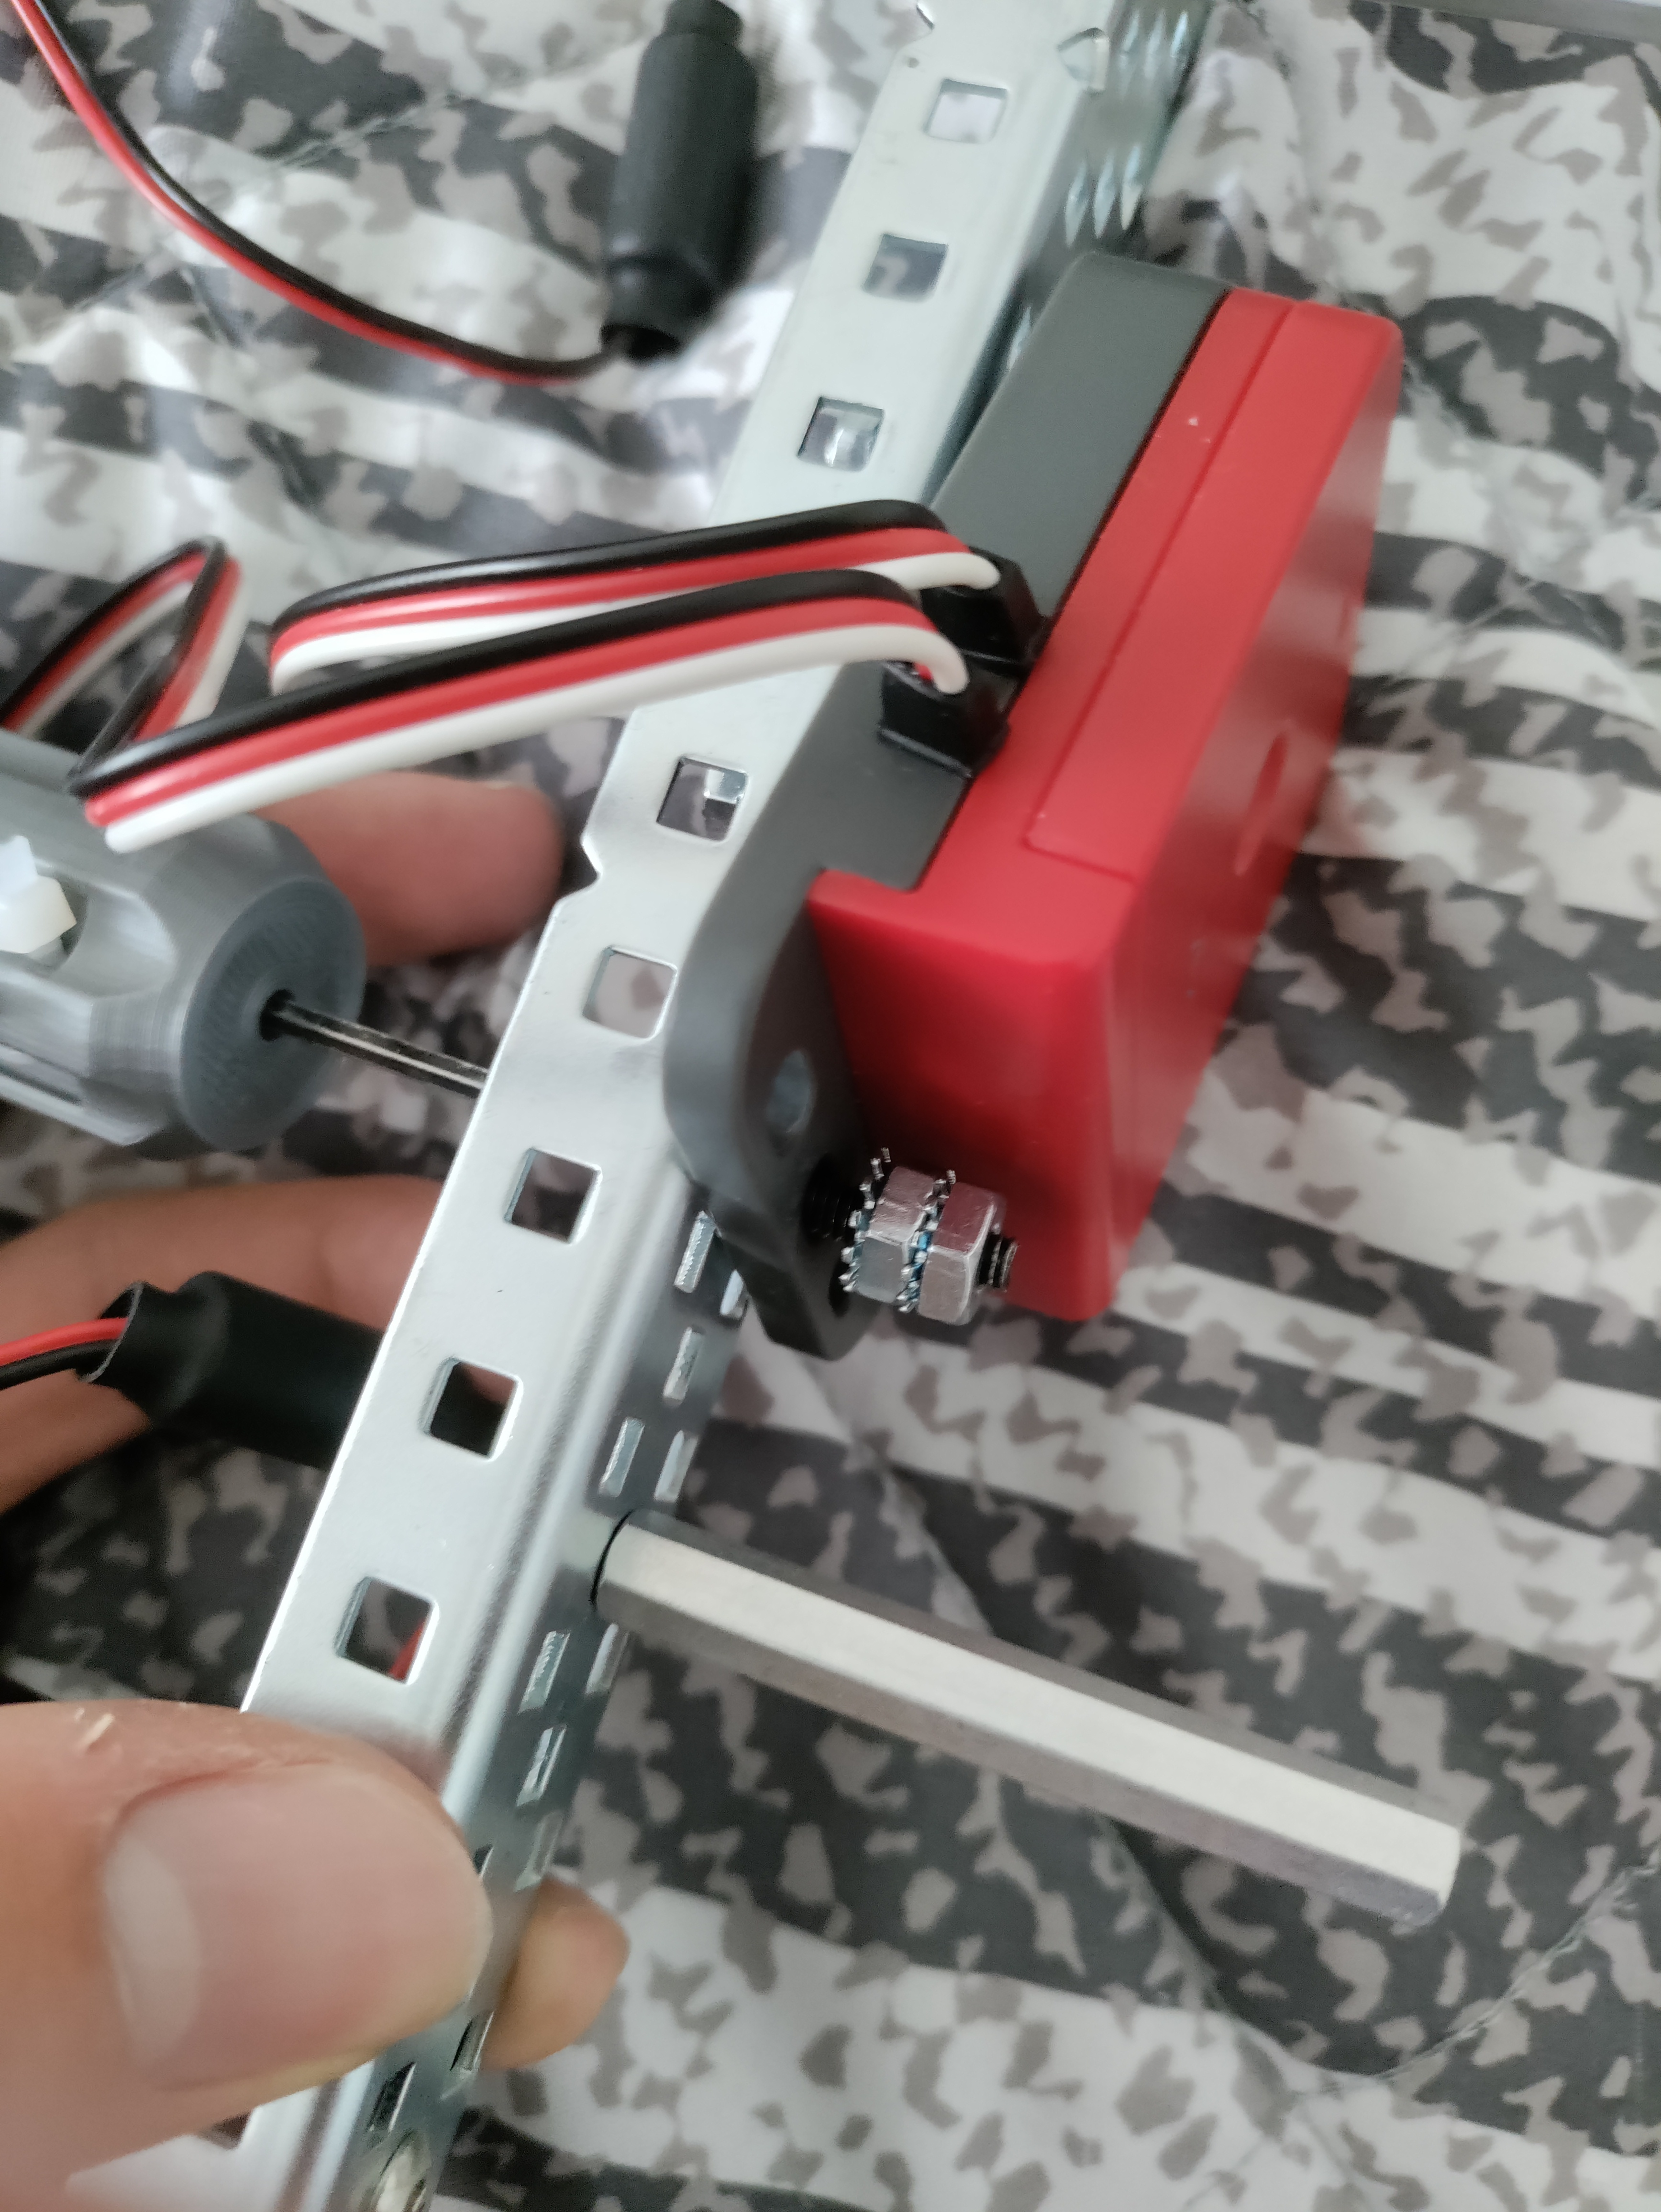
\includegraphics[width=\textwidth,height=9cm,keepaspectratio=true]{ScrewAxle}
    \caption{
        A single screw axle being used to attach an encoder to the chassis. The encoder is free to move up and down in the case of axle vibration, and the screw axle prevents it from going anywhere else.
    }
\end{figure}
